Kiến trúc vi dịch vụ có nhiều ưu điểm, đặc biệt với các dự án có quy mô lớn và phức tạp.

\begin{itemize}

    \item Kiến trúc vi dịch vụ phân chia dự án thành các dịch vụ nhỏ.

          \begin{itemize}

              \item Giúp việc phát triển và quản lý hệ thống dễ dàng hơn.

              \item Tận dụng sử dụng tài nguyên theo nhu cầu cho từng dịch vụ riêng.


          \end{itemize}
    \item Các dịch vụ độc lập về nghiệp vụ kinh doanh.
    
    Các nhóm không cần hiểu sâu về mọi khả năng kinh doanh.      Dẫn tới tốc độ phát triển thay đổi nhanh và   tốc độ định giá doanh nghiệp nhanh hơn.
    
    \item Các dịch vụ độc lập về         ngôn ngữ lập trình và CSDL
    \begin{itemize}

        \item     Kiến trúc vi dịch vụ sử dụng đa ngôn ngữ và công nghệ khác nhau. Từ đó tận dụng hiệu quả thế mạnh của từng ngôn ngữ, công nghệ phù hợp nhất cho yêu cầu nghiệp vụ cụ thể.   

        \item        Giảm chi phí và thời gian kiểm thử do ít ràng buộc.
        \item Ví dụ: Mỗi dịch vụ sử dụng ngôn ngữ lập trình nhau khác như: NodeJS, Go, Python, Java, CSharp,...
        
        
        
         
        \begin{figure}[h] 
        \centering
        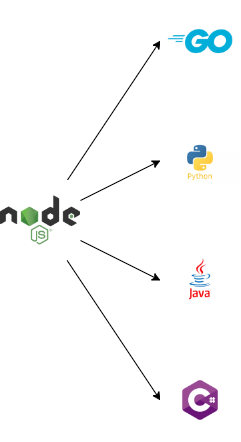
\includegraphics[height=3cm]{pictures/DaNgonNgu/_DaNgonNgu.png}
        \caption{ViDuHinhAnhTheoChieuDoc}  
        % % Thêm vào hình SQL riêng 
        \end{figure} 
        
       


        
        
        


    \end{itemize}
\end{itemize}

%     \item Các  
% 
%                         %     $VD: 




%                           \item Độc lập về     triển khai hệ thống



%                           Mỗi dịch vụ   triển khai độc lập và có thể thực hiện các thay đổi  mà không ảnh hưởng đến các dịch vụ khác.  





%           \end{itemize}
% \end{itemize}

% % Các dịch vụ ít phụ thuộc vào các dịch vụ khác.
% Giảm thiểu ràng buộc và tăng tính linh hoạt của hệ thống.
% Hệ thống có khả năng chịu lỗi cao tăng độ tin cậy.
% % Khả năng phục hồi : Kiến trúc phải được thiết kế để chịu đựng lỗi và các dịch vụ phải có khả năng xử lý lỗi một cách duyên dáng.
% Tính linh hoạt : Kiến trúc phải cho phép phát triển và triển khai nhanh chóng các dịch vụ mới cũng như khả năng thay đổi các dịch vụ hiện có một cách nhanh chóng và dễ dàng.
% \textbf{Từ đó    dễ dàng  mở rộng hệ thống.}
%%%%%%%%%%%%%%%%%%%%%%%%%%%%%%%%%%%%%



%%%%%%%%%%%%%%%%%%%%%%%%%%%%%%%%%%%%%


% Các dịch vụ tương tác với nhau qua hạ tầng mạng.

% Các dịch vụ tương tác với nhau qua hạ tầng mạng.

% Các dịch vụ tương tác với nhau qua hạ tầng mạng.

% Các dịch vụ tương tác với nhau qua hạ tầng mạng.

% Các dịch vụ tương tác với nhau qua hạ tầng mạng.

% Các dịch vụ tương tác với nhau qua hạ tầng mạng.

% Các dịch vụ tương tác với nhau qua hạ tầng mạng.

% Các dịch vụ tương tác với nhau qua hạ tầng mạng.

% Các dịch vụ tương tác với nhau qua hạ tầng mạng.